% !TEX TS-program = pdflatex
% !TEX encoding = UTF-8 Unicode

% This is a simple template for a LaTeX document using the "article" class.
% See "book", "report", "letter" for other types of document.

\documentclass[11pt]{scrartcl} % use larger type; default would be 10pt

\usepackage[utf8]{inputenc} % set input encoding (not needed with XeLaTeX)

%%% Examples of Article customizations
% These packages are optional, depending whether you want the features they provide.
% See the LaTeX Companion or other references for full information.

%%% PAGE DIMENSIONS
\usepackage{geometry} % to change the page dimensions
\geometry{a4paper} % or letterpaper (US) or a5paper or....
% \geometry{margin=2in} % for example, change the margins to 2 inches all round
% \geometry{landscape} % set up the page for landscape
%   read geometry.pdf for detailed page layout information

\usepackage{graphicx} % support the \includegraphics command and options

% \usepackage[parfill]{parskip} % Activate to begin paragraphs with an empty line rather than an indent

%%% PACKAGES
\usepackage{booktabs} % for much better looking tables
\usepackage{array} % for better arrays (eg matrices) in maths
\usepackage{paralist} % very flexible & customisable lists (eg. enumerate/itemize, etc.)
\usepackage{verbatim} % adds environment for commenting out blocks of text & for better verbatim
\usepackage{subfig} % make it possible to include more than one captioned figure/table in a single float
\usepackage{graphicx}
% These packages are all incorporated in the memoir class to one degree or another...

%%% SECTION TITLE APPEARANCE
\usepackage{sectsty}
\allsectionsfont{\sffamily\mdseries\upshape} % (See the fntguide.pdf for font help)
% (This matches ConTeXt defaults)

%%% ToC (table of contents) APPEARANCE
\usepackage[nottoc,notlof,notlot]{tocbibind} % Put the bibliography in the ToC
\usepackage[titles,subfigure]{tocloft} % Alter the style of the Table of Contents
\renewcommand{\cftsecfont}{\rmfamily\mdseries\upshape}
\renewcommand{\cftsecpagefont}{\rmfamily\mdseries\upshape} % No bold!


\usepackage{amssymb}
\usepackage{amsmath}
\usepackage{mathcomp}
%\usepackage{colortbl}
\usepackage{dsfont}
\usepackage{amsfonts}
\usepackage{cancel}

%%% KV-Diagramme
%\usepackage[ngerman]{babel}
\input kvmacros

%%% Graphen
\usepackage{tikz}
\usetikzlibrary{intersections}
\usetikzlibrary{calc}

% last page
\usepackage{pageslts}

%%% END Article customizations

%%% HEADERS & FOOTERS
\usepackage{fancyhdr} % This should be set AFTER setting up the page geometry
%\usepackage{scrpage2} % Another package (only use fancyhdr or scrpage2)
\pagestyle{fancy} % options: empty , plain , fancy
\renewcommand{\headrulewidth}{1.2pt} % customise the layout...
\renewcommand{\footrulewidth}{0.1pt} % customise the layout...
\lhead{MACHINE LEARNING 1\\Andres Fernandez -- 5692442 -- fr\_andres@msn.com}\chead{}\rhead{Exercise Sheet 3 \\November 21, 2016}
\lfoot{}\cfoot{\thepage/\lastpageref{LastPages}}\rfoot{}



%%% THE SYMBOLS FOR ``DEPENDENT'' AND ``INDEPENDENT''
\newcommand{\CI}{\mathrel{\text{\scalebox{1.07}{$\perp\mkern-10mu\perp$}}}} % independent
\newcommand{\nCI}{\cancel{\mathrel{\text{\scalebox{1.07}{$\perp\mkern-10mu\perp$}}}}} % dep
%% THE SYMBOL FOR DOESN'T IMPLY
\newcommand{\notimplies}{%
  \mathrel{{\ooalign{\hidewidth$\not\phantom{=}$\hidewidth\cr$\implies$}}}}

%%% The "real" document content comes below...


\begin{document}

\section*{\\[3mm]Exercise 1}
         {\it Consider a multivariate normal distribution in variable \(x\) with mean \(\mu\) and covariance \(\Sigma\). Show that if we make the linear transformation \(y=Ax+b\) then the transformed variable y is distributed as:
           \begin{align*}
             p(y) = \mathcal{N}(A\mu+b, A\Sigma A^T)
         \end{align*}}
  

         \subsection*{i)}
         Asked is then to show that the normal distribution of an affine transformation is a normal distribution itself, with the mentioned transformations applied to its parameters. For that sake it is necessary to remember the definition of the multivariate normal function (for a positive, semi-definite covariance matrix \(\Sigma\)):
         \begin{equation}\label{eq:1}
           \mathcal{N}(\vec{x} | \vec{\mu}, \Sigma) =\frac{1}{\sqrt{|2\pi\Sigma|}}
           \exp\left(-\frac{1}{2}(\vec{x}-\vec{\mu})^T{\Sigma}^{-1}(\vec{x}-\vec{\mu})\right)
         \end{equation}

         And substituting it with the corresponding affine transformation yields the following formula (the vector arrows will be from now on omitted):
        \begin{equation}\label{eq:2}
           \mathcal{N}({Ax+b} | {\mu}, \Sigma) = \frac{1}{\sqrt{|2\pi\Sigma|}} \exp\left(-\frac{1}{2}({(Ax+b)}-{\mu})^T{\Sigma}^{-1}({(Ax+b)}-{\mu})\right)
         \end{equation}

        %% It is important to recall that, given \(x, \mu \in\mathbb{R}^D\) and \(\Sigma \in \mathbb{R}^{D\times D}\), the following must be also true:
        %% \begin{equation}\label{eq:2}
        %%    b \in\mathbb{R}^D\) \quad and \quad \(A \in \mathbb{R}^{D\times D}
        %%  \end{equation}

         %% \begin{equation}
         %%   \begin{split}
         %%     &\frac{1}{\sqrt{|2\pi\Sigma|}} \exp\left(-\frac{1}{2}({(Ax+b)}-{\mu})^T{\Sigma}^{-1}({(Ax+b)}-{\mu})\right)\\
         %%     &= \frac{1}{\sqrt{|2\pi(A\Sigma A^T)|}}\exp\left(-\frac{1}{2}({x}-{(A\mu+b}))^T{(A\Sigma A^T)}^{-1}({x}-{(A\mu+b)})\right)\\
         %%   \end{split}
         %% \end{equation}


         \subsection*{ii)}
         In order to reduce equation \ref{eq:2}, the following properties of linear algebra are assumed:

         \begin{equation}
           \begin{split}
             &(A^{-1})^T = (A^{T})^{-1} = A A^{-T}\\
             &(AB)^T = B^TA^T\\
             &(AB)^{-1} = B^{-1}A^{-1}\\
             &A^{-1} A = A^T A^{-T} = I\\
             &IA = AI = A\\
             & y=Ax+b \iff x=A^{-1}(y-b)
           \end{split}
         \end{equation}

         This assumptions are valid for a matrix A of any size, having the identity matrix \(I\) the corresponding number of dimensions in each case.

         \subsection*{iii)}
         Now it's possible to perform the transformation in the body of the exponential function:
         \begin{equation}
           \begin{split}
              (x-{\mu})^T&{\Sigma}^{-1}(x-{\mu}) =\\
             ({(A^{-1}(y-b))}-{\mu})^T&{\Sigma}^{-1}({(A^{-1}(y-b))}-{\mu}) =\\
             ({(A^{-1}(y-b))}-{\mu})^T \mathbf{(A^T&A^{-T})}{\Sigma}^{-1}\mathbf{(A^{-1}A)}({(A^{-1}(y-b))}-{\mu})=\\
             \left(({(A^{-1}(y-b))}-{\mu})^T A^T\right)&\mathbf{\left(A^{-T}\Sigma^{-1} A^{-1} \right)} \left( A({(A^{-1}(y-b))}-{\mu})\right)=\\
             \mathbf{\left(A({A^{-1}(y-b))}-{\mu}\right)^T}&\left(A^{-T}\Sigma^{-1} A^{-1} \right) \mathbf{\left({(AA^{-1}(y-b))}-{A\mu}\right)}=\\
             \mathbf{(y-b-A\mu)^T}&\left(A^{-T}\Sigma^{-1} A^{-1} \right) \mathbf{(y-b-{A\mu})}=\\
             (y-\mathbf{(A\mu+b)})^T&\mathbf{(A\Sigma A^T)^{-1}} (y-\mathbf{(A\mu+b)})\\
           \end{split}
         \end{equation}
         Whereas \(A^{-T}\Sigma^{-1} A^{-1} = A^{-T}(A\Sigma)^{-1} = A\Sigma A^T^{-1}\). Also, recall that the normalization factor remains the same regardless of the dimensions of A, since it depends only on the original \(\Sigma\). Therefore, the following equivalence holds:


         \begin{equation}
           \begin{split}
             \rho(x)=\rho(A^{-1}(y-b)) = &\frac{1}{\sqrt{|2\pi\Sigma|}} \exp\left(-\frac{1}{2}(y-\mathbf{(A\mu+b)})^T\mathbf{(A\Sigma A^T)^{-1}} (y-\mathbf{(A\mu+b)}))\right) = \\
             &= \mathcal{N}(y | A\mu+b, A\Sigma A^T)\\
           \end{split}
         \end{equation}
         
         \begin{flushright}
           $\square$\\
         \end{flushright}

         

\vspace{5mm}
\section*{Exercise 2}
         {\it Show that we can convert a normal distribution with mean \(\mu\) and covariance \(\Sigma\) to a new distribution with mean \(0\) and covariance \(I\) using the linear transformation \(y = Ax+b\) where
           \begin{align*}
             A= \Sigma^{-\frac{1}{2}}\\
             b=-\Sigma^{-\frac{1}{2}}\mu
           \end{align*}

         This is known as the whitening transform. Note that \(M\) is the square root of a matrix \(Q\), i.e. \(M = Q^{\frac{1}{2}}\) , if \(M M = Q\)}

         
         \subsection*{i)}
         Here, the following linear algebra assumptions are needed:
         \begin{equation}
           \begin{split}
             &I\cdot I = I \iff I^{-1} = I\\
             &A^{-\frac{1}{2}}A^{-\frac{1}{2}} = A^{-1}\\
             &A^{-\frac{1}{2}}A^{\frac{1}{2}} = I\\
             &\Sigma= \Sigma^T \iff \Sigma^{-1}= \Sigma^{-T} \iff \Sigma^{\frac{1}{2}}= (\Sigma^{\frac{1}{2}})^T\\
             &A^{-\frac{1}{2}}A^{\frac{1}{2}} = I\\
           \end{split}
         \end{equation}
         And also the following implication: \(y=Ax+b \iff x = A^{-1}(y-b)\), which, for the given values, yields:
         \begin{align*}
           x = (\Sigma^{-\frac{1}{2}})^{-1}(y-(-\Sigma^{-\frac{1}{2}}\mu)) = \Sigma^{\frac{1}{2}}(y+\Sigma^{-\frac{1}{2}}\mu) = \Sigma^{\frac{1}{2}}y +\mu
         \end{align*}

         \subsection*{ii)}
         Now, substituting in the exponential body of the normal PDF,
         \begin{equation}
           \begin{split}
             &\exp\left(-\frac{1}{2}((\Sigma^{\frac{1}{2}}y+\mu)-\mu)^T{\Sigma}^{-1}((\Sigma^{\frac{1}{2}}y+\mu)-\mu)\right) =\\
             &\exp\left(-\frac{1}{2}(\Sigma^{\frac{1}{2}}y)^T{\Sigma}^{-1}(\Sigma^{\frac{1}{2}}y)\right) =\\
             &\exp\left(-\frac{1}{2}(\Sigma^{\frac{1}{2}}y)^T{\Sigma}^{-\frac{1}{2}}{\Sigma}^{-\frac{1}{2}}(\Sigma^{\frac{1}{2}}y)\right)=\\
             &\exp\left(-\frac{1}{2}(y^T(\Sigma^{\frac{1}{2}})^T{\Sigma}^{-\frac{1}{2}}({\Sigma}^{-\frac{1}{2}}\Sigma^{\frac{1}{2}}y)\right)=\\
             &\exp\left(-\frac{1}{2}(y^Ty)\right)=\exp\left(-\frac{1}{2}((y-0)^TI(y-0))\right)\\
           \end{split}
         \end{equation}
         Which yields a normal distribution with zero value for \(\mu\) and the identity matrix for \(\Sigma\).\\


         \vspace{5mm}
\section*{Exercise 3}
         {\it Now, we want to exploit the knowledge acquired in Exercises 1 and 2 to conceive a method for sampling random vectors from an arbitrary multivariate normal distribution \(\mathcal{N}(\mu, \Sigma)\). Sampling from a distribution means, the probability of drawing a given vector is proportional to the pdf of this distribution. First, we sample a vector of length \(N\) (number of dimensions) from a normal distribution \(\mathcal{N}(0, I)\). Since all components are uncorrelated, we can easily do this by drawing \(N\) random numbers using a built-in random number generator for univariate normal distributions. Then we transform the samples with appropriate matrix \(B\), such that the new distribution has the desired covariance. Finally, we shift the samples to the desired mean value \(v\).}        
         \subsection*{a) How are \(B\), \(\Sigma\) and \(v\) related?}
         If I understood correctly, the described setup intends to achieve the transformation from a standard normal multivariate distribution \(x_1\sim\mathcal{N}(0, I)\) to any other multivariate distribution \(x_2\sim\mathcal{N}(\mu, \Sigma)\), by application of the affine transformation \(y=Bx+v\).\\
         Based on the relations showed before, we know that \(y\sim\mathcal{N}(B\cdot 0 +v, B\cdot I \cdot B^T) = \mathcal{N}(v, BB^T)\). Therefore,
         \begin{align*}
           \begin{split}
             &v\text{ becomes directly the new expected value, that is: }v=\mu\\
             &BB^T\text{ becomes the new covariance matrix }\Sigma.\\
             &\text{ If B is a triangular and square matrix, this is the \textbf{Cholesky decomposition}.}
           \end{split}
         \end{align*}
         \subsection*{b) Sample 1000 values from the two-dimensional normal distribution with mean vector \(\mu= \begin{pmatrix} 2 \\ 3 \end{pmatrix}\), and the covariance matrix \(\Sigma = \begin{pmatrix}
             4 &  -0.5 \\-0.5 & 2 \\\end{pmatrix}\). Plot a two-dimensional histogram and explain why this plot shows approximately the desired distribution. Use \(M\times M\) quadratic bins of equal size. The value of a given bin is defined as the number of samples that fall into this bin, divided by the total number of samples. To plot the histogram, represent bin values by grey values (or color) and plot these grey values into a two-dimensional coordinate system (like an 'image')}
         See Figure \ref{fig2}, and see/run the Python2 script {\it fernandez\_blatt3.py} for the details. 
         \begin{figure}[ht]
	   \centering
           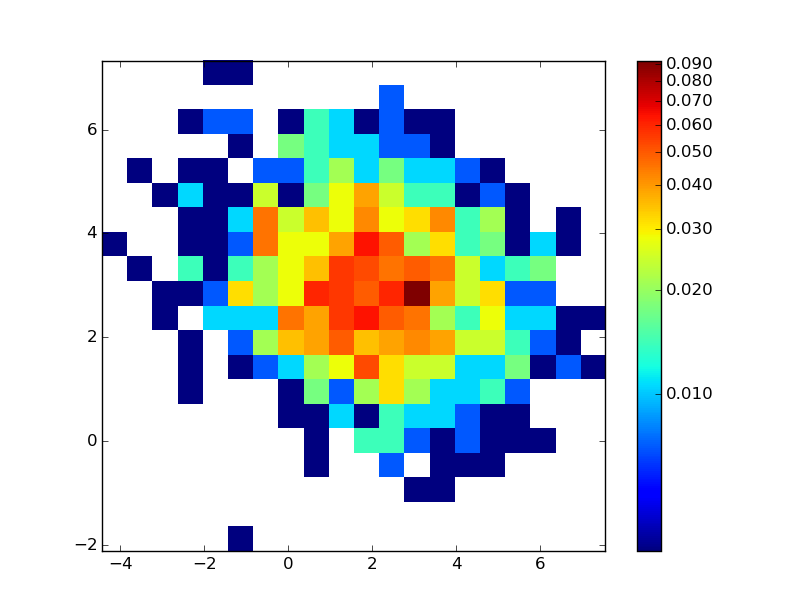
\includegraphics[width=0.6\textwidth, angle=0]{multivar_1.png}
	   \caption{2D-histogram for 20x20 bins, 1000 samples}
	   \label{fig2}
         \end{figure}
         This plot shows approximately the desired distribution, because the ``color density'' is maximal around the given \(\mu\) value, and it decreases exponentially. Furthermore, the standard deviation of the horizontal axis is bigger than the vertical one, and they are negatively correlated, as stated in the \(\Sigma\) matrix.
         \subsection*{c) Estimate the mean and covariance matrix from the data using their Maximum Likelihood estimates. How close are the estimated parameters to the real ones? Use 2, 20, 200 data points for your estimate}
         Run the attached Python2 script to generate similar results:\\[2mm]
         estimated cov(x, y) for 1000 samples: -0.345968387603\\[2mm]
         estimated mean of x for 2 samples: 4.82419813156\\
         estimated mean of y for 2 samples: 2.10856773405\\
         estimated variance of x for 2 samples: 0.518180558768\\
         estimated variance of y for2 samples: 0.00268184920367\\
         estimated cov(x, y) for 2 samples: 0.0745568808063\\[2mm]
         estimated mean of x for 20 samples: 1.87527441792\\
         estimated mean of y for 20 samples: 3.26096396479\\
         estimated variance of x for 20 samples: 2.04668336757\\
         estimated variance of y for20 samples: 2.05992159961\\
         estimated cov(x, y) for 20 samples: -0.0237578274471\\[2mm]
         estimated mean of x for 200 samples: 2.18152415943\\
         estimated mean of y for 200 samples: 3.17357837903\\
         estimated variance of x for 200 samples: 3.45526621455\\
         estimated variance of y for200 samples: 1.8364091909\\
         estimated cov(x, y) for 200 samples: -0.405670949001\\

         
         \subsection*{Plot the likelihood as a function of two parameters of your choice, keeping all other parameters constant}
         The likelihood function for a given set of one-dimensional points \(x_1, ..., x_N\) is:
         \begin{equation}\label{eq:8}
               \begin{split}
                 \mathcal{L}(\mu, \sigma^2, x_1, ..., x_N) = (2\pi\sigma^2)^{-\frac{n}{2}}exp\left(-\frac{1}{2\sigma^2}\sum_{i=1}^N\{(x_i-\mu)^2\} \right)
               \end{split}
             \end{equation}
         Since it returns a scalar, it can also easily be expanded to multidimensional points by adding the likelihood of each dimension. Since likelihood is mostly meaningful based on a sample set, it makes sense to calculate a fixed set of points, and take the expected value and variance as variables:
         \begin{figure}[ht]
	   \centering
           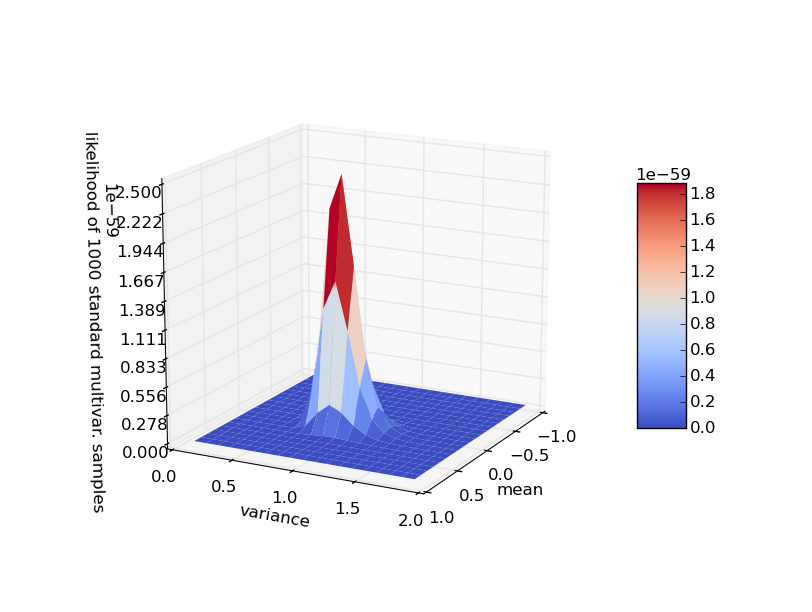
\includegraphics[width=1\textwidth, angle=0]{likelihood.png}
	   \caption{Likelihood of 1000 standard,multivariate, normal distributed samples}
	   \label{fig2}
         \end{figure}


\end{document}
